\section{Test/Resultater}

\subsection{Bremse-test}

For at teste effekten af bremsen, opstillede vi en lang lige bane, for at afprøve bilens bremselængde. Bremselængde skulle gerne variere alt efter, hvor lang tid motoren var kortsluttet. Vi satte bilen igang med samme hastighed og varierede kortslutningsperioderne i intervallerne 0, 50, 100, 200, 300, 400 og 500 millisekunder. Når bilen krydsede målstregen, slukkedes motoren og bremsen blev tilsluttet. Så lod vi bilen køre indtil den stoppede og målte afstanden til målstregen. Hver periode blev kørt fem gange og så beregnede vi gennemsnittet. Testen blev lavet for tre forskellige værdier i OCR2 - 255, 180 og 120 svarende til duty cycles på henholdsvis 100 \%, 70,6 \% og 47 \% (se figur \ref{fig:Bremselir}. 

\begin{figure}[h]

	\centering
		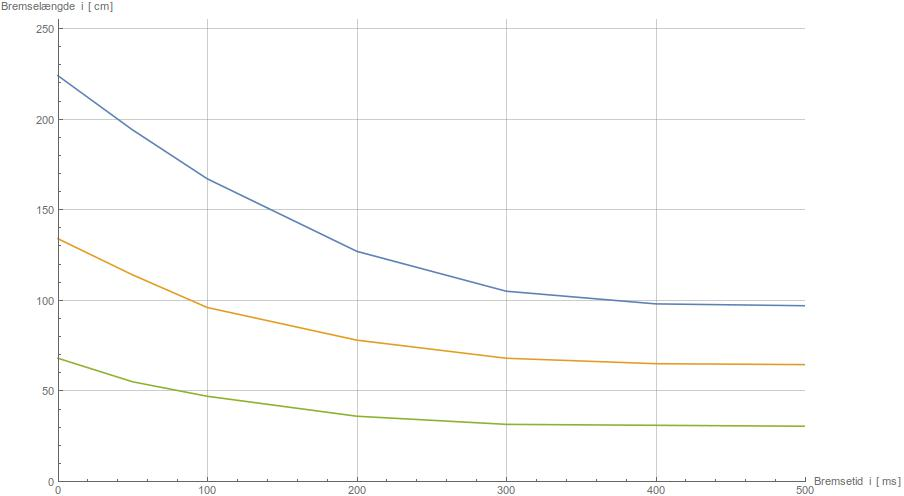
\includegraphics[scale=0.4]{Billeder/Bremse.jpeg}
	\caption{Her ses bremselængden i forhold til bremsetiden, med bremselængden i cm op ad y-aksen, og bremsetiden i ms ud ad x-aksen}
	\label{fig:Bremselir}
	
\end{figure}

Ud fra testen kan vi konkludere at bremsen har størst effekt ved korte bremsetider under 300 ms.

\subsection{Mapping-test}

